%-----------------------------------------------------------
\section{Visuels Python / R : usages, atouts, limites}
\label{sec:python-r-visuals}
%-----------------------------------------------------------

Outre les visuels préfabriqués, Power BI autorise l’exécution de scripts Python ou R pour produire des visuels sur mesure.  
L’utilisateur insère un composant « Python visual » ou « R visual » dans le canevas, saisit le code dans un éditeur intégré, puis Power BI exécute ce script en tâche de fond : les données liées sont transmises sous forme de DataFrame et le résultat retourné est une image statique (PNG) affichée dans le rapport.

Cette fonctionnalité exploite l’écosystème analytique complet de chaque langage : Matplotlib, Seaborn ou Plotly côté Python ; ggplot2 ou plotly R côté R.  
Un data-scientist peut, en quelques lignes, tracer dans Power BI un nuage de points avec régression \textsc{Loess} (R) ou un diagramme de réseau (Python) — visuels impossibles à obtenir via les graphes natifs, notamment quand l’Arbre de décomposition limite la profondeur d’analyse et n’accepte qu’une seconde mesure \parencite{MicrosoftDecompositionTree2024}.

\begin{figure}[h]
  \centering
  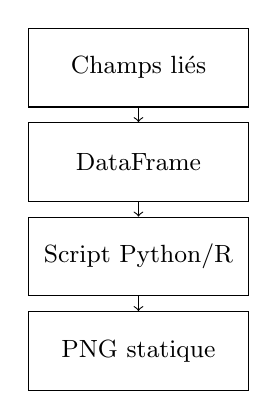
\begin{tikzpicture}[node distance=1.2cm, every node/.style={font=\small}]
    \node (bind) [draw, rectangle, minimum width=2.8cm, minimum height=1cm] {Champs liés};
    \node (df)   [below of=bind, draw, rectangle, minimum width=2.8cm, minimum height=1cm] {DataFrame};
    \node (code) [below of=df,   draw, rectangle, minimum width=2.8cm, minimum height=1cm] {Script Python/R};
    \node (png)  [below of=code, draw, rectangle, minimum width=2.8cm, minimum height=1cm] {PNG statique};
    \draw[->] (bind) -- (df);
    \draw[->] (df)   -- (code);
    \draw[->] (code) -- (png);
  \end{tikzpicture}
  \caption{Pipeline d’exécution d’un visuel Python / R dans Power BI}
  \label{fig:python-r-pipeline}
\end{figure}

\subsection{Atouts analytiques}

L’accès direct aux bibliothèques open-source autorise statistiques avancées, clustering, apprentissage automatique, carte de chaleurs ou dendrogrammes ; le script peut pré-traiter les données ou entraîner un modèle avant de générer le graphique.  
À chaque rafraîchissement, l’exécution se relance automatiquement : l’utilisateur bénéficie ainsi de calculs que DAX ou Power Query ne permettent pas aisément, par exemple l’analyse de texte ou les séries temporelles non linéaires.

\subsection{Limites techniques et fonctionnelles}

Le résultat demeure une image statique — « les visualisations Python dans Power BI sont des bitmaps 72 DPI, sans interactivité directe » \parencite{MicrosoftPythonRVisualsDocs2024}.  
Impossible donc d’initier un filtrage croisé depuis le graphique ; seul un filtre externe relance le script.  
Power BI transmet au script au plus 150 000 lignes, alloue 250 Mio de mémoire et impose un temps plafond de cinq minutes en local, soixante secondes dans le service ; la sortie PNG des visuels R est limitée à 2 Mio \parencite{MicrosoftRPackagesService2025}.  
Le runtime cloud, actuellement R 4.3.3 et Python 3.11, restreint le package compressé à 30 Mio, et l’affichage de ces visuels exige une licence Pro ou un workspace Premium : un utilisateur Free ne les verra pas.

\subsection{Enjeux de sécurité et de maintenance}

Power BI signale explicitement qu’un visuel Python ou R contient du code exécutable arbitraire \parencite{MicrosoftPythonRVisualsDocs2024}.  
Dans un environnement professionnel, cela impose une gouvernance rigoureuse : le script, encapsulé dans le fichier binaire .pbix, échappe au suivi Git ; il doit donc être extrait dans un dépôt versionné afin de permettre la traçabilité et la revue par les pairs. De plus, le runtime cloud (Python 3.11, R 4.3.3) ainsi que ses bibliothèques sont mis à jour automatiquement chaque mois ; un fichier requirements.txt (ou renv.lock pour R) et des tests de régression sont indispensables pour vérifier la compatibilité après chaque release. Enfin, puisque ces scripts disposent d’un accès direct au système de fichiers et au réseau, il convient de restreindre leurs privilèges (comptes de service à droits minimaux, liste blanche de packages) afin de prévenir toute exfiltration de données ou exécution de code malveillant.

\subsection{Bilan et positionnement stratégique}

Les visuels Python et R offrent un recours efficace pour des analyses spécialisées ponctuelles, mais la nature statique du rendu, les contraintes de performance et les exigences de licence limitent leur usage à grande échelle.  
Une comparaison détaillée entre visuels natifs, Python/R et SDK figurera dans le tableau synthétique de la section \ref{sec:synthese}; on y montrera que, pour un besoin récurrent et interactif, le développement d’un visuel SDK représente l’alternative la plus pérenne pour ECRINS SA.
